


\section{Frontend}

\subsection{Navigation}

For navigation the following libraries were used:
\begin{lstlisting}
"react-navigation": "^4.0.10",
"react-navigation-drawer": "^2.3.3",
"react-navigation-stack": "^1.10.3",
"react-navigation-tabs": "^2.7.0",
\end{lstlisting}

As you can see in the code provided below, app starts with a splash screen (which was implemented by the following  tutorial at:  

\url{ https://medium.com/handlebar-labs/how-to-add-a-splash-screen-to-a-react-native-app-ios-and-android-30a3cec835ae)}


\begin{lstlisting}
const MyApp = createSwitchNavigator({
        loading: {
            screen: SplashScreen
        },
        app: appDrawer,
        auth: authStack
    },
    {
        initialRouteName: 'loading'
    })

const AppNavigation = createAppContainer(MyApp);

\end{lstlisting}

In SplashScreen component the saved email and token from the local storage are sent to the server, which compares it with its data and sends a response back. Depending on the response (valid/invalid) it navigates either to authentication or application route correspondingly.

There are 3 stacks in navigation: Authentication, Drawer and Tabs Stacks.
Authentication consists of 2 components: Login and Register.

Drawer or "hamburger" menu has Profile, Settings and Log out options.

There are 2 bottom tabs: 'Feed' and 'My City'.

Main components and navigation between them is shown in the diagram below Fig.~\ref{fig:Navigation Diagram}


\subsubsection{Authentication Stack}
Consists of 2 components:

1. Login

2. Register

In order to use the app user has to register first. 
After logging in (or first registration) server assigns a token to the user.
Next time if the user has not logged out (just closed the app) then there is no necessity to log in again. Token and email get saved in local storage of a phone, after launching the app they are sent to the server, which checks if they are valid or not (if such email and token exist). 
If a user logs out then 'token-email pair' get erased from the local storage and the server and user has to log in again.

Screenshots of register and login pages are shown below in Fig.~\ref{fig:Register} and Fig.~\ref{fig:Login}

\subsubsection{App Stack}

\textbf{1. Drawer}

As illustrated in Fig.~\ref{fig:Drawer} drawer contains user profile information, settings and an option to log out alongside with user's avatar and user's current geolocation. In more detail about each component further below.

$\bullet Profile$

Profile contains user's avatar, geolocation, email, name and description. Apart from that, there are two carousels of visited cities and visited places. A user can add a city or a place to 'visited list' by pressing a check-box icon at the top right corner in City details or Place details page.

There is an option to edit profile, which navigates to settings component, described further.

$ \bullet Settings$

Allows to modify name and description. Avatar can be changed either in drawer or in profile by clicking on the image and uploading a new one.

$\bullet Log out$

As mentioned before calls logout method in authentication server, which clears token assigned to email when logging in (as well as clears it from local storage).

\textbf{2. Tabs }

Bottom tab navigation contains Feed (with all the cities' info) and My City (city, identified by the geolocation).

$ \bullet Feed$
Displays all cities created, posts, places and posts about the places. 

$ \bullet My City$
Displays a city information, a user is currently in and posts about that city.


\subsection{Client-Server Communication}
As described in Methodology chapter client 'communicates' with the Server using GRPC.

There are 4 services: 

1. Authentication
- required for login and register.

2. Post Service
- for retrieving, creating and updating posts.

3. Profiles Service
- for retrieving, creating and updating cities, places and users.

4. Photos Service
- responsible for all the images.

In order to establish communication between client and server as shown in Fig.~\ref{fig:Client-Server Communication Diagram} a 'bridge' between Android native and JavascriptCore was required to be built.

2 classes were written per each service:

Client.java - a class that calls stub methods.

Module.java - a class which calls methods of Client.java. 
IP address and port number are specified here as well.


\

Note: Each module needs to be added to a package. All packages have to be added to the List<ReactPackage> in MainApplication.java

In javascript code a NativeModules library has to be imported.

\begin{lstlisting}
import { NativeModules} from 'react-native';
\end{lstlisting}

\begin{figure}[ht]
    \centering
    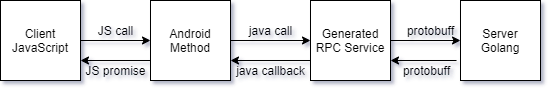
\includegraphics[width=0.9\textwidth]{img/client-server.png}
     \caption{Client-Server Communication Diagram}
    \label{fig:Client-Server Communication Diagram}
\end{figure}


\begin{figure}[ht]
    \centering
    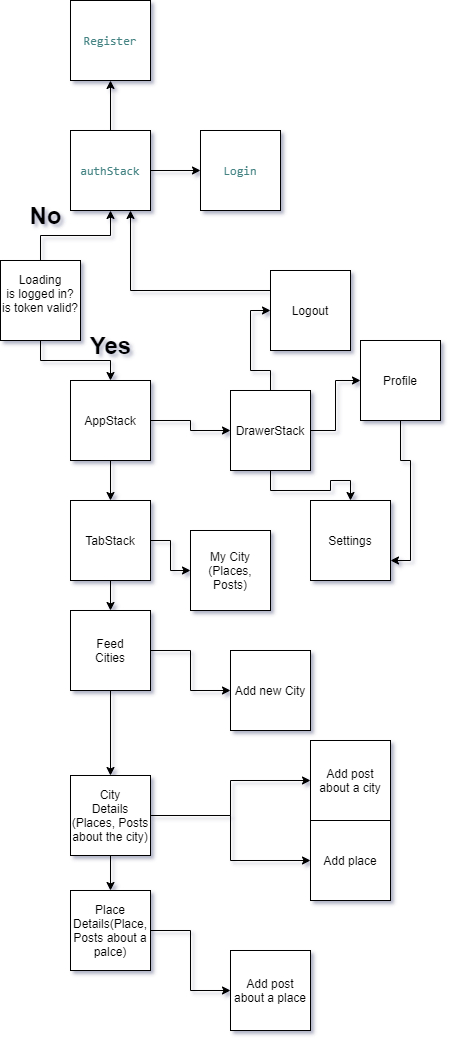
\includegraphics[width=0.5\textwidth]{img/nav_diagram .png}
     \caption{Navigation Diagram}
    \label{fig:Navigation Diagram}
\end{figure}



\subsection{Prototypes}
Fig.~\ref{fig:Login Prototype} -~\ref{fig:Home Page Prototype} represent some of the prototype pages, final UI (screenshots) can be found in the next chapter.

\begin{figure}[h!]
\begin{minipage}[t]{0.48\textwidth}
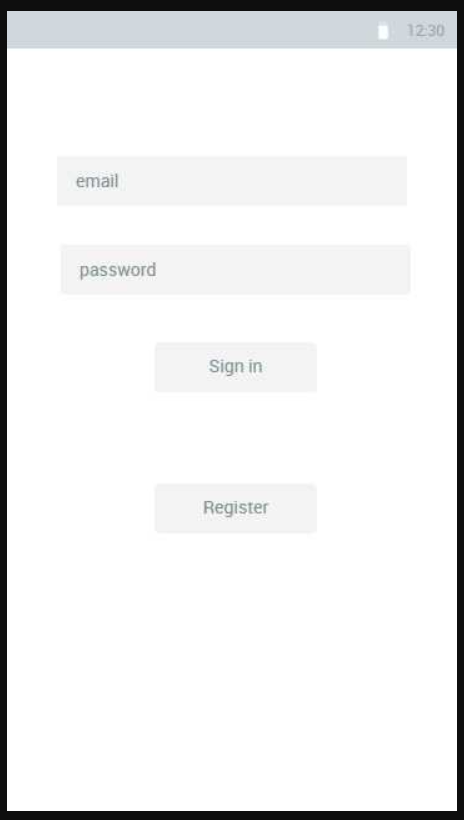
\includegraphics[width=\linewidth,keepaspectratio=true]{img/login_mock.PNG}
\caption{Login Prototype}
\label{fig:Login Prototype}
\end{minipage}
\hspace*{\fill} % it's important not to leave blank lines before and after this command
\begin{minipage}[t]{0.48\textwidth}
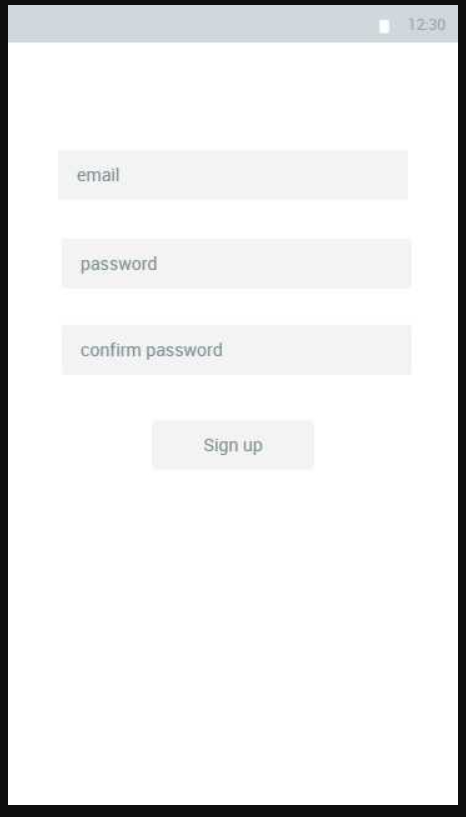
\includegraphics[width=\linewidth,keepaspectratio=true]{img/register_mock.PNG}
\caption{Register Prototype}
\label{fig:Register Prototype}
\end{minipage}
\end{figure}


\begin{figure}[h!]
\begin{minipage}[t]{0.48\textwidth}
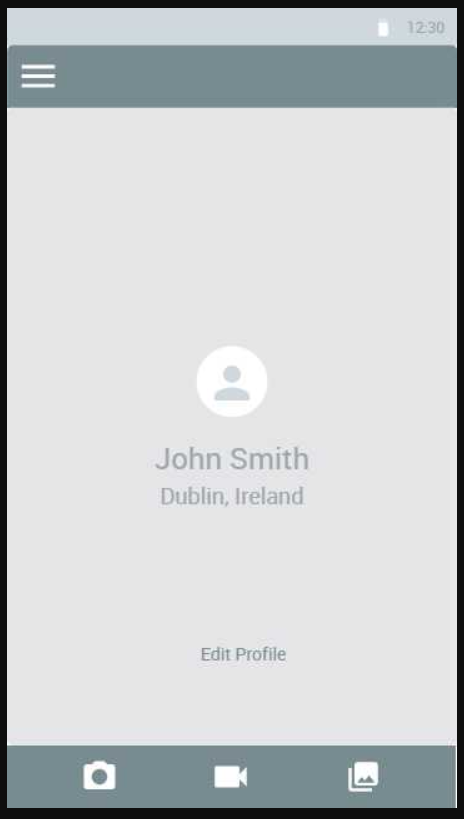
\includegraphics[width=\linewidth,keepaspectratio=true]{img/profile_mock.PNG}
\caption{Profile Prototype}
\label{fig:Profile Prototype}
\end{minipage}
\hspace*{\fill} % it's important not to leave blank lines before and after this command
\begin{minipage}[t]{0.48\textwidth}
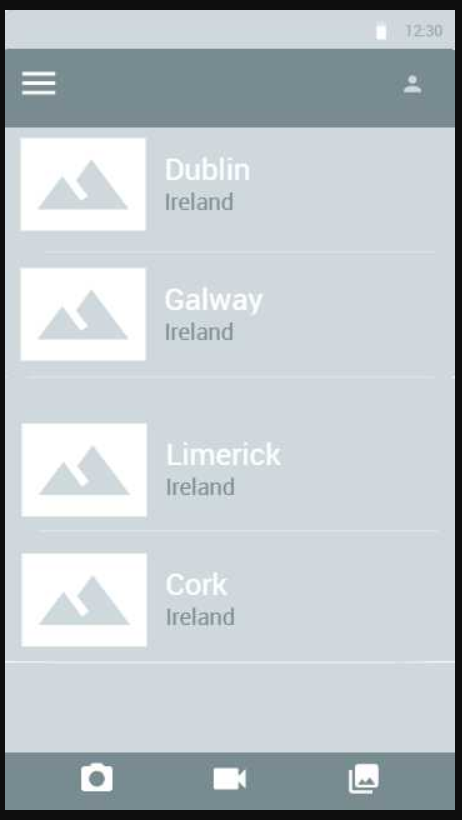
\includegraphics[width=\linewidth,keepaspectratio=true]{img/home_page_mock.PNG}
\caption{Home Page Prototype}
\label{fig:Home Page Prototype}
\end{minipage}
\end{figure}